\chapter{Implementación}


A la hora de implementar esta nueva arquitectura debemos considerar que, para ejecutarla, hay que crear un entorno, un escenario, real sobre el que hacerlo. O, en su defecto, crear un entorno que simule esas condiciones para trabajar con ella.


Es por ello que antes de trabajar con el modelo de ``Swiftnet'' \cite{swiftnet} tenemos que sentar las bases sobre las que se pueda ejecutar. Así comienza la creación de un entorno Conda.

\section{Conda}

Conda \cite{conda} es un sistema de gestión de entornos con el que creamos el escenario sobre el que vamos a correr ``Swiftnet'' \cite{swiftnet}. Conda permite crear el escenario instalando y gestionando paquetes de uso público ubicados en diferentes ``canales'' del sistema. Simplemente hay que seguir las instrucciones que dan para descargarlos e instalarlos, y poder añadirlos así al escenario sobre el que se esté trabajando.

\begin{figure}[H]
  \centering
  
\includegraphics[width=8cm]{Figuras/Conda.eps}
  \caption{Conda}
\end{figure}

Antes de crear ningún entorno, primero hay que instalar Conda en la máquina que va a procesar el proyecto. Para ello descargamos Miniconda (un instalador de Conda) para Python 2.7 \cite{miniconda_install}. Una vez descargado ya podemos crear entornos Conda.


Para crear el entorno Conda sobre el que trabajar basta con abrir un terminal del sistema operativo y escribir el siguiente comando:

\begin{center}
\textit{conda  create  --name  swiftnet  python=3.7}
\end{center}

En este caso estamos creando un entorno Conda llamado ``swiftnet'' con la versión de Python 3.7 (la necesaria para el modelo de ``Swiftnet'', aunque se admiten versiones superiores  \cite{github_swiftnet}).


Ya tenemos creado el entorno, ahora hace falta añadirle los paquetes necesarios que requiere ``Swiftnet'', indicados en el archivo ``requirements.txt'' \cite{github_swiftnet}. Para instalarlos simplemente seguimos las indicaciones del modelo y usamos este comando:

\begin{center}
\textit{pip install -r requirements.txt}
\end{center}

``Pip'' es otro gestor de paquetes que, junto a Conda, es muy útil a la hora de instalar aquellos paquetes que Conda no posee en sus ``canales'' \cite{pip}.

Con el anterior comando, se instalan una serie de paquetes necesarios para la ejecución del modelo, entre ellos PyTorch \cite{pytorch}, del cual hablaremos más adelante; pero no todos (en nuestro caso). Para que el modelo funcione correctamente hay que instalar los restantes con este comando \cite{conda_sheet}:

\begin{center}
\textit{conda install nombre\_del\_paquete -c nombre\_del\_canal\_en\_el\_que\_se\_encuentra\_el\_paquete}
\end{center}

A continuación enumeramos los paquetes que quedan para poder ejecutar ``Swiftnet'':

\begin{enumerate}
\item opencv \cite{opencv}
\item pytorch torchaudio=0.4.0 cudatoolkit=10.0 \cite{pytorch}
\end{enumerate}

Cabe destacar que ponemos dichos paquetes con estas versiones porque las especificaciones de nuestra máquina lo requerían. Si se quiere reproducir el resultado de este proyecto, puede que no sean las mismas versiones de estos paquetes los que haya que instalar, dependerá de la máquina sobre la que se trabaje.

Una vez instalados dichos paquetes, se sigue el procedimiento marcado por el modelo y se ejecuta desde el directorio en el que éste se encuentra:

\begin{center}
\textit{python eval.py configs\textbackslash{rn18\_single\_scale.py}}
\end{center}

Tras ello, y en nuestro caso particular, se llegarán a dos errores:

\begin{enumerate}
\item No se encuentra el módulo ``lib.cylib''
\item No se encuentra la versión ``GLIBCXX\_3.4.26'' de ``libstdc++'' que se encuentra en el sistema operativo
\end{enumerate}

Pasamos a explicarlos:

\subsection{Error de ``lib.cylib''}

Este error se da porque aún no se ha creado módulo de ``cython'' \cite{cython} necesario para evaluar las métricas del modelo. Se consigue ejecutando el código del archivo ``build.sh'' del modelo en la carpeta ``lib\textbackslash{}'' de éste.

Sin embargo, antes de ejecutarlo conviene modificarlo de la siguiente manera:

\begin{figure}[H]
  \centering
  \includegraphics[width=8cm]{Figuras/cylib.eps}
  \caption{Archivo ``build.sh''}
  \label{fig:cylib}
\end{figure}

Tras hacerlo, lo ejecutamos con el siguiente comando:

\begin{center}
\textit{.\textbackslash{build.sh}}
\end{center}

Si nos sale algún error porque falta algún paquete por instalar, volvemos al comando que utilizamos para instalar paquetes por Conda y los instalamos de forma sencilla.

Como se puede observar en la figura \ref{fig:cylib}, el archivo está en ``Shell Script'' \cite{shell} y a través de éste se crean los archivos ``cylib.so'', ``cylib.cc'' y ``cylib.html''.

Cabe destacar otra observación muy importante en la figura: Hay que modificar las líneas en las que se hace referencia al sistema de archivos propio de la máquina sobre la que se trabaja.

En nuestro caso, tenemos la siguiente ruta sequida de los directorios que se han creado al haber instalado los paquetes previos a la ejecución del modelo:

\begin{center}
\textit{\textbackslash{home}\textbackslash{sergios}\textbackslash{miniconda2}\textbackslash{envs}\textbackslash{swiftnet}}
\end{center}

Es muy importante cambiar esa ruta por la de la máquina sobre la que se trabaje, si no, no puede funcionar; de modo que cuando se instale Conda y se cree el entorno sobre el que se quiere trabajar, hay que tener en cuenta esta especificación.

Por otro lado, el resto de la ruta no se modifica, ya que son paquetes comunes a cualquier usuario que intente ejecutar ``Swiftnet'' \cite{swiftnet}.

Por último, puntualizar que la última parte comentada del archivo, que es muy similar a la que hemos modificado hace un momento, sirve para lo mismo pero utilizando Python 3.8. Si se quisiese utilizar este modelo con esa versión de Python habría que descomentarla y comentar la referente a Python 3.7.

\subsection{Error de ``GLIBCXX''}

Para empezar, ``libstdc++'' \cite{glibcxx} es la implementación de la librería estándar del lenguaje C++ de programación.

Esto quiere decir que para cualquier programa en C++ que use hilos o archivos, por ejemplo, usará esta librería para implementar lo pertinente a estas cosas en las librerías de C++.

Por otro lado tenemos la \ac{ABI} \cite{glibcxx}, la cual sirve para que, por ejemplo, un programa compilado en ``libstdc++'' en 2013 funcione de la misma manera para una nueva versión de ``libstdc++'' en 2021. Cuando se actualiza esa librería y se quiere compilar un programa de una versión anterior, se mantiene la ABI de dicha versión para compilar ese programa.

Sin embargo, cuando se actualiza ``libstdc++'' y se mantiene su ABI, cada función o símbolo de dicha librería obtiene una nueva versión, a la que se le llama mediante un ``linker''.

El ``linker'' enlaza la llamada a una función de la librería con su última versión \cite{glibcxx}.

Para nuestro caso, no encuentra la versión ``GLIBCXX\_3.4.26'' de ``libstdc++'' debido a que el ``linker'' no tiene permisos para acceder a la librería del sistema operativo. Por lo que, cada vez que ejecutemos el modelo, aunque lo intente, no podrá encontrar dicha librería.

Sin embargo, he aquí una razón de uso de los entornos Conda: Cuando se crea un entorno Conda nuevo, éste también adquiere esta librería al venir incluida en uno de los paquetes de instalación predeterminados para la creación del entorno. De este modo obtenemos la versión que requiere ``Swiftnet'' para su ejecución.

Aún así sigue existiendo un problema: el ``linker'' sigue buscando la versión requerida por ``Swiftnet'' en el mismo lugar, de modo que cada vez que se llame a esa librería el ``linker'' seguirá buscando donde siempre y seguiremos igual. La solución reside en hacerle saber al ``linker'' dónde buscar esta nueva versión, y para ello usaremos este comando en la terminal:

\begin{center}
\textit{export LD\_LIBRARY\_PATH=\$LD\_LIBRARY\_PATH:\$HOME\textbackslash{miniconda2}\textbackslash{lib}\textbackslash{}}
\end{center}

No obstante, esta solución sirve siempre y cuando no se cierre la terminal. En el momento en el que se cierre hay que volver a abrir otra y volver a utilizarlo.

Al usarla, conseguimos nuestro objetivo y podemos seguir avanzando en la ejecución del modelo.

\section{PyTorch}





